\documentclass[a4,11pt]{article}

\usepackage{graphicx}
\usepackage[labelfont=bf]{caption}
\usepackage{subcaption}
\usepackage{fancyhdr}
\usepackage{hyperref}
\usepackage[utf8]{inputenc}
\setlength{\headheight}{13.6pt}

\lhead
\rhead
\parskip 1em
\parindent 0em

\begin{document}
\pagestyle{empty}
%-----------------------------------------------------------
\begin{titlepage}

	\title{\Huge{Lab report} \\[0.1cm] \Large{Digital Design (EDA322)} \\[0.4cm]}
	\author{\large{\emph{Group 9, Tuesday AM}} \\[0.2cm] Dennis Bennhage \\[0.05cm] Hampus Lidin \\[0.1cm]}
	\maketitle
	\thispagestyle{empty}
\end{titlepage}
\clearpage
%-----------------------------------------------------------
\pagestyle{fancyplain}
\pagenumbering{roman}
\tableofcontents
\clearpage
%%%%%%%%%%%%%%%%
% Introduction
\pagenumbering{arabic}
\setcounter{page}{1}
\section{Introduction}
(max: 1 page)
\\\\
This part will introduce the reader to the report. 

At the beginning, describe what the purpose of this lab report is. Then describe briefly what each section discusses and finally summarise the most important conclusions. 

\section{Method}
The processor was designed in VHDL-code, using software QuestaSim (ModelSim) for simulation and
XillinxISE for synthesizing. 

\subsection{Arithmetic and Logic Unit (ALU)}

The ALU can take two 8-bit unsigned data words, and perform either of the following operations:
addition, subtraction, bitwise NAND or bitwise NOT. It also has four indicators: {\it Carry},
{\it isOutZero}, {\it Eq} and {\it NotEq}. The {\it Carry}-bit sets to 1 when an overflow occurs
(note that this indicator is only valid when performing addition). The other indicators are
self-explanatory. When choosing what operation to perform on the inputs, you set the two-bit
{\it operation} signal to one of the codes specified in Table~\ref{tab:op}.

We started out with implementing the data flow architecture for a {\it full adder}. A full adder
takes three bits of input, where two of them are the numbers being added and the third one is a
{\it carry-in}, as shown in Figure~\ref{fig:fa}. If at least 2 of the inputs are set to 1, a
{\it carry-out} will be set. The sum output is the remainder of the addition of the three inputs.
With this implementation, we were able to construct a {\it ripple carry adder}, using 8 full adders.
The ripple carry adder could then be used for addition and subtraction in the final ALU-component.
The reader can find the block diagram for the ripple carry adder in Figure~\ref{fig:rca} in
Appendix~\ref{app:fig}.

We had to implement additional circuitry for handling the subtraction of the two inputs. For
that we first defined an internal signal {\it SUB}, that entirely depends on the first bit of the
operation signal. We also defined an 8-bit internal signal, that depends on the {\it exclusive
or} between the second ALU-input and the {\it SUB}-signal. In that way, when the {\it SUB}-signal
is set, the {\it XOR}-gate behaves like an inverter. With the inverted input and the {\it SUB}-signal
going directly to the carry-in of the first full adder, we have the {\it 2 compliment} of the second
input, which is just what is needed for the subtraction to work (see Figure~\ref{fig:sub} in
Appendix~\ref{app:fig} for the block diagram).

Finally, we needed to implement the data flow for a 4-1 {\it multiplexer}, whose purpose is to
select the correct operation for the ALU-output. We did this in VHDL-code by matching the operation
signal to it's corresponding operation, and then sending the signal to the output.

\begin{table}   
	\centering
	\small
	\def\arraystretch{1.1}              
	\begin{tabular}{|l|l|}
		\hline
		{\it Operation} & {\bf Operation} \\ \hline
		00              & Addition        \\ 
		01              & Subtraction     \\
		10              & Bitwise NAND    \\ 
		11              & Bitwise NOT     \\ \hline
	\end{tabular}
	\caption{The operation codes for choosing an ALU-operation.}
	\label{tab:op}
\end{table}

\begin{figure}[h!]
	\centering
 	\begin{subfigure}{.5\textwidth}
		\centering
		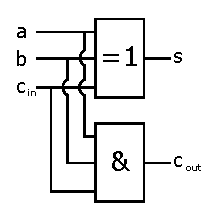
\includegraphics[height=.3\textheight]{Figurer/fa}
		\caption{A full adder.}
		\label{fig:fa} 
	\end{subfigure}%
	\begin{subfigure}{.5\textwidth}
		\centering
		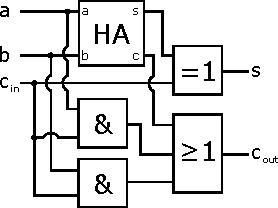
\includegraphics[height=.3\textheight]{Figurer/fa2}
		\caption{A full adder using a half adder.}
		\label{fig:fa2} 
  	\end{subfigure}
	\caption{Figure~\ref{fig:fa} shows the data flow implementation of a full adder,
		and Figure~\ref{fig:fa2} shows the alternative structural design using a half adder.}
\end{figure}

\newpage

\subsection{Top-level Design}
(max: 2 pages)
\\\\
Describe what you did in lab 3. In addition, describe how you implemented the bus using the mux and any extra logic or the tri-state buffers. Describe briefly how you implemented the storage elements that are used by the ChAcc processor. Show one snapshot of the simulation waveform where you write something to a memory location and then read from it. Remember to always explain your design choices and mention any assumptions. Finally, make use of figures and tables. 

\subsection{Controller}
(max: 2 pages)
\\\\
Describe what you did in lab4. More specifically, show the \emph{Finite-state machine} (FSM) of the controller by presenting the diagram you drew. Which design decisions did you make and why? Also include few waveforms, where you show that the controller runs correctly for some particular instructions using the provided testbench. Remember to always explain your design choices and mention any assumptions. Finally, make use of figures and tables. 

\subsection{Processor's Testbench}
(max: 2 pages)
\\\\
Describe what you did in lab5. More specifically, describe how you made the testbench to verify that your processor design was functionally correct. For example, you can specify how you generated inputs to the processor during the testing, how you were reading the expected outputs and how you compare the expected outputs with the actual outputs. Also mention if your processor design was working correctly from the beginning and if not describe how you backtrack the bugs. Remember to always explain your design choices and mention any assumptions. Finally, make use of figures and tables. 

\subsection{ChAcc on Nexys 3 board \emph{(Optional)}}
(max: 2 pages)
\\\\
Describe how you verified the correctness of your FPGA implementation. Note that the code that is executed on the implementation is the same code used for testing in Lab 5. You should compare sequences of values on various signals observed on the seven-segment displays to values seen in Modelsim simulation of the design. Please include in the report the sequence of program counter (PC) and display register values you observed during a successful execution on the FPGA. 

\subsection{Performance, Area and Power Analysis \emph{(Optional)}}
(max: 2 pages)
\\\\
To be announced in the Lab7PM.

\section{Analysis}
(max: 1 page)
\\\\
Summarize your results after performing all the labs (2, 3, 4 and 5).

Mention and discuss interesting findings and observations, as well as difficulties in completing some of the tasks of the four last labs.

After looking at your results, draw conclusions and describe briefly the learning outcome, that is what have you learnt by performing these labs?  

% Appendix
\newpage
\begin{appendix}

\section{Figures}
\label{app:fig}

\begin{figure}[h!]
 	\centering
	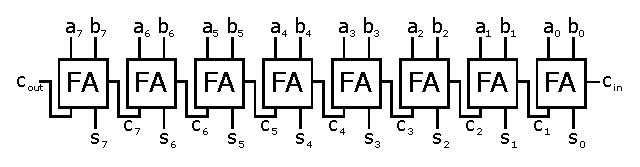
\includegraphics[width=1\columnwidth]{Figurer/rca}
  	\caption{A structural implementation of an 8-bit ripple carry adder using eight full adders.}
  	\label{fig:rca}
\end{figure}

\begin{figure}[h!]
 	\centering
	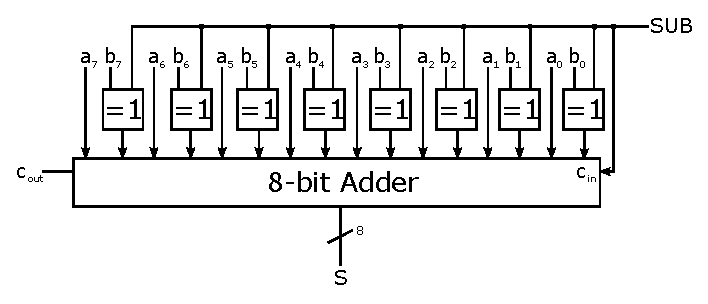
\includegraphics[width=1\columnwidth]{Figurer/sub}
  	\caption{Additional circuitry that is needed in order for the subtraction
		operation to work.}
  	\label{fig:sub}
\end{figure}

\end{appendix}

\end{document}
